\chapter{Testing}
In the chapter aspects of dynamic white box testing will be explained in Section \vref{sec:DynamicWhiteBoxTesting}.
Furthermore the results of the usability test will be presented in Section \vref{sec:usability_results}.

\section{Dynamic White Box Testing}
\label{sec:DynamicWhiteBoxTesting}
To ensure the correctness of the Oasis Lib we enforced dynamic white box testing through unit tests \cite[pp106]{Testing} \cite{UnitTesting}.
The Oasis Lib is used by all GIRAF applications this means that if a bug exists in the Oasis Lib there is a potential bug in all GIRAF applications.
Therefore the Oasis Lib must be thoroughly tested to make sure that few or no bugs exists.

The Oasis Local Db will be tested along with the Oasis Lib, this is more efficient as more code will be tested in every test, but it has the drawback that if a bug appears more code will have to be investigated in order to locate the bug.

As this project have been developed using the agile development method Scrum we have not devised a full test plan as this is not needed \cite[pp263]{Testing}. 
The focus of the tests will be on test-to-pass \cite[pp66]{Testing}.
This ensures that the Oasis Lib will function as intended, though there is no guarantee that the Oasis Lib will work if invalid parameters are used.

\subsection{The Test Designs}
\label{sec:testDesign}
A test design have been elaborated for each method in the helper classes of the Oasis Lib \cite[pp281]{Testing}.
Examples of the test designs are presented in the following tables.

The test design in Table \vref{tab:TestDesign_AuthenticateProfile} is for the \texttt{authenticateProfile()} method.
This test design tests if a profile can be authenticated.
This is an essential method for the GIRAF platform, and therefore it is tested both using test-to-pass and test-to-fail tests to ensure that this method is particular robust.

\begin{table}[H]
	\centering
		\begin{tabular}{| p{4.5cm} | m{9cm} |}
			\hline
			\textbf{Identifier:} 				& TD00001 \\ \hline
			\textbf{Feature to be tested:}		& Authenticate profile. \\ \hline
			\textbf{Approach:}					& An automated test will be made to authenticate a profile by its certificate. \\
												&	\begin{enumerate}
														\item Enter a profile with a specific certificate in the database.
														\item Authenticate the profile by its certificate.
													\end{enumerate} \\ \hline
			\textbf{Test case identification:} 	& Check valid certificate Test Case ID\# 00001 \\
												& Check too long certificates Test Case ID\# 00002 \\
												& Check too short certificates Test Case ID\# 00003 \\
												& Check invalid certificates Test Case ID\# 00004 \\ \hline
			\textbf{Pass/fail criteria:}			& All valid profile certificates that matches the certificate in the database must be accepted as well as all invalid certificates must be rejected. \\ \hline
		\end{tabular}
	\caption{Test Design for \texttt{authenticatingProfile()}.}
	\label{tab:TestDesign_AuthenticateProfile}
\end{table}

The test design in Table \vref{tab:TestDesign_GetProfileById} is for the \texttt{getProfileById()} method.
This is also an important method for the GIRAF system, therefore it is tested with the same mix of test-to-pass and test-to-fail tests.
The tests ensures the robustness of the method.

\begin{table}[H]
	\centering
		\begin{tabular}{| p{4.5cm} | m{9cm} |}
			\hline
			\textbf{Identifier:}				& TD00002 \\ \hline
			\textbf{Feature to be tested:}		& Get profile by id. \\ \hline
			\textbf{Approach:}					& An automated test will be made in order to ensure that the Oasis Library supports getting a profile by its id from the database. \\
												&	\begin{enumerate}
														\item Add Profiles to the database.
														\item Get profile by id and verify the output.
												\end{enumerate} \\ \hline
			\textbf{Test case identification:}	& Check valid id present in the database Test Case ID\# 00005 \\
												& Check id not in the database Test Case ID\# 00006 \\
												& Check negative id Test Case ID\# 00007 \\ \hline
			\textbf{Pass/fail criteria:}		& The profile matching the id should be returned else null should be returned. \\ \hline
		\end{tabular}
	\caption{Test Design for \texttt{getProfileById()}.}
	\label{tab:TestDesign_GetProfileById}
\end{table}

The test design in Table \vref{tab:TestDesign_GetChildrenByGuardian} is for the \texttt{getChildrenByGuardian()} method.
The test ensures the method performs as intended under normal operation.
This is done with a single test-to-pass test, which tests if children associated to a guardian can be retrieved from the database.

\begin{table}[H]
	\centering
		\begin{tabular}{| p{4.5cm} | m{9cm} |}
			\hline
			\textbf{Identifier:} 				& TD00003 \\ \hline
			\textbf{Feature to be tested:}		& Get children by guardian. \\ \hline
			\textbf{Approach:}					& An automated test will be made to ensure that the Oasis Library supports getting all children associated with one guardian. \\
										&	\begin{enumerate}
												\item Children and guardians should be added to the database.
												\item Associations between some children and guardians should be made.
												\item Get children by guardian should be called and the output verified.
											\end{enumerate} \\ \hline
			\textbf{Test case identification:} 	& Check valid guardian with children associated Test Case ID\# 00008 \\ \hline
			\textbf{Pass/fail criteria:}			& The list of children should match the children associated with the guardian. \\ \hline
		\end{tabular}
	\caption{Test Design for \texttt{getChildrenByGuardian}.}
	\label{tab:TestDesign_GetChildrenByGuardian}
\end{table}



\subsection{The Test Cases}
For each test design in Section \vref{sec:testDesign}, one or more test cases has been created \cite[pp283]{Testing}.
Each test case ensures a part of the tested method performs as intended in the test situation.
The test cases for the test designs presented in Section \vref{sec:testDesign} will be shown in the following tables:
Table \vref{tab:TestCase_ValidCertificateHandling}, 
Table \vref{tab:TestCase_CertificateToShortHandling},
Table \vref{tab:TestCase_CertificateToLongHandling},
Table \vref{tab:TestCase_InvalidCertificateHandling},
Table \vref{tab:TestCase_ValidIdHandling},
Table \vref{tab:TestCase_InvalidIdHandling},
Table \vref{tab:TestCase_NegativeIdHandling}, 
and Table \vref{tab:TestCase_ValidGuardianWithChildrenAssociatedHandling}.

\begin{table}[H]
	\centering
		\begin{tabular}{| p{4.5cm} | m{9cm} |}
			\hline
			\textbf{Identifier:} 					& TC00001 \\ \hline
			\textbf{Test item:}						& Valid Certificate handling of the \texttt{authenticateProfile()} method. \\ \hline
			\textbf{Input specification:}			& A valid certificate. \\ \hline
			\textbf{Output specification:} 			& The model of the authenticated profile. \\ \hline
			\textbf{Environmental needs:}			& A database is needed and the profile model. \\ \hline
			\textbf{Special procedural requirements:}	& None. \\ \hline
			\textbf{Intercase dependencies:}			& None. \\ \hline
		\end{tabular}
	\caption{Test Case for valid certificate handling of the \texttt{authenticateProfile()} method.}
	\label{tab:TestCase_ValidCertificateHandling}
\end{table}

\begin{table}[H]
	\centering
		\begin{tabular}{| p{4.5cm} | m{9cm} |}
			\hline
			\textbf{Identifier:} 					& TC00002 \\ \hline
			\textbf{Test item:}						& Certificate length too short handling of the \texttt{authenticateProfile()} method. \\ \hline
			\textbf{Input specification:}			& A certificate shorter than 200 chars. \\ \hline
			\textbf{Output specification:} 			& Null. \\ \hline
			\textbf{Environmental needs:}			& A database is needed and the profile model. \\ \hline
			\textbf{Special procedural requirements}	& None. \\ \hline
			\textbf{Intercase dependencies:}			& None. \\ \hline
		\end{tabular}
	\caption{Test Case for certificate length too short handling of the \texttt{authenticateProfile()} method.}
	\label{tab:TestCase_CertificateToShortHandling}
\end{table}

\begin{table}[H]
	\centering
		\begin{tabular}{| p{4.5cm} | m{9cm} |}
			\hline
			\textbf{Identifier:} 					& TC00003 \\ \hline
			\textbf{Test item:}						& Certificate length too long handling of the \texttt{authenticateProfile()} method. \\ \hline
			\textbf{Input specification:}			& A certificate longer than 200 chars. \\ \hline
			\textbf{Output specification:} 			& Null. \\ \hline
			\textbf{Environmental needs:}			& A database is needed and the profile model. \\ \hline
			\textbf{Special procedural requirements:}	& None. \\ \hline
			\textbf{Intercase dependencies:}			& None. \\ \hline
		\end{tabular}
	\caption{Test Case for certificate length too long handling of the \texttt{authenticateProfile()} method.}
	\label{tab:TestCase_CertificateToLongHandling}
\end{table}

\begin{table}[H]
	\centering
		\begin{tabular}{| p{4.5cm} | m{9cm} |}
			\hline
			\textbf{Identifier:} 					& TC00004 \\ \hline
			\textbf{Test item:}						& Invalid Certificate handling of the \texttt{authenticateProfile()} method. \\ \hline
			\textbf{Input specification:}			& An invalid certificate. \\ \hline
			\textbf{Output specification:} 			& Null. \\ \hline
			\textbf{Environmental needs:}			& A database is needed and the profile model. \\ \hline
			\textbf{Special procedural requirements:}	& None. \\ \hline
			\textbf{Intercase dependencies:}			& None. \\ \hline
		\end{tabular}
	\caption{Test Case for invalid certificate handling of the \texttt{authenticateProfile()} method.}
	\label{tab:TestCase_InvalidCertificateHandling}
\end{table}

\begin{table}[H]
	\centering
		\begin{tabular}{| p{4.5cm} | m{9cm} |}
			\hline
			\textbf{Identifier:} 					& TC00005 \\ \hline
			\textbf{Test item:}						& Valid id present in the database handling of the \texttt{getProfileById()} method. \\ \hline
			\textbf{Input specification:}			& A valid id. \\ \hline
			\textbf{Output specification:} 			& The profile matching the id. \\ \hline
			\textbf{Environmental needs:}			& A database is needed and the profile model. \\ \hline
			\textbf{Special procedural requirements:}	& None. \\ \hline
			\textbf{Intercase dependencies:}			& None. \\ \hline
		\end{tabular}
	\caption{Test Case for valid id handling of the \texttt{getProfileById()} method.}
	\label{tab:TestCase_ValidIdHandling}
\end{table}

\begin{table}[H]
	\centering
		\begin{tabular}{| p{4.5cm} | m{9cm} |}
			\hline
			\textbf{Identifier:} 					& TC00006 \\ \hline
			\textbf{Test item:}						& Invalid id not present in the database handling of the \texttt{getProfileById()} method. \\ \hline
			\textbf{Input specification:}			& An invalid id. \\ \hline
			\textbf{Output specification:} 			& Null. \\ \hline
			\textbf{Environmental needs:}			& A database is needed and the profile model. \\ \hline
			\textbf{Special procedural requirements:}	& None. \\ \hline
			\textbf{Intercase dependencies:}			& None. \\ \hline
		\end{tabular}
	\caption{Test Case for invalid id handling of the \texttt{getProfileById()} method.}
	\label{tab:TestCase_InvalidIdHandling}
\end{table}

\begin{table}[H]
	\centering
		\begin{tabular}{| p{4.5cm} | m{9cm} |}
			\hline
			\textbf{Identifier:} 					& TC00007 \\ \hline
			\textbf{Test item:}						& Negative id handling of the \texttt{getProfileById()} method. \\ \hline
			\textbf{Input specification:}			& A negative id. \\ \hline
			\textbf{Output specification:} 			& Null. \\ \hline
			\textbf{Environmental needs:}			& A database is needed and the profile model. \\ \hline
			\textbf{Special procedural requirements:}	& None. \\ \hline
			\textbf{Intercase dependencies:}			& None. \\ \hline
		\end{tabular}
	\caption{Test Case for negative id handling of the \texttt{getProfileById()} method.}
	\label{tab:TestCase_NegativeIdHandling}
\end{table}

\begin{table}[H]
	\centering
		\begin{tabular}{| p{4.5cm} | m{9cm} |}
			\hline
			\textbf{Identifier:} 					& TC00008 \\ \hline
			\textbf{Test item:}						& Valid guardian with children associated handling of the \texttt{getChildrenByGuardian()} method. \\ \hline
			\textbf{Input specification:}			& A valid guardian. \\ \hline
			\textbf{Output specification:} 			& A list of associated children. \\ \hline
			\textbf{Environmental needs:}			& A database is needed and the profile model. \\ \hline
			\textbf{Special procedural requirements:}	& None. \\ \hline
			\textbf{Intercase dependencies:}			& None. \\ \hline
		\end{tabular}
	\caption{Test Case for valid guardian with children associated handling of the \texttt{getChildrenByGuardian()} method.}
	\label{tab:TestCase_ValidGuardianWithChildrenAssociatedHandling}
\end{table}


\subsection{Unit Test Implementation}
All the tests cases have been used to construct the 89 unit tests, which have helped in the development of the Oasis Lib.
The tests have been split up into three parts; initialization, execution, and assertion.

The unit test for the \texttt{testAuthenticateProfileWithValidCertificate()} method can be seen in Listing \vref{lst:testAuthenticateProfileWithValidCertificate}.
The method starts by initializing the environment.
This means that a random valid certificate is created and a profile -- the expected profile -- is entered in the database and the certificate for the profile is set to the newly created certificate.

After the initialization the method is executed and the retrieved profile is stored as the actual profile in order to have some data for the assertion.
At the end an \texttt{assertEquals} is called to ensure that the expected profile is the same as the actual profile.
If this is the case the test passes, otherwise the test fails and the two profiles are printed in the test log. 


\begin{Java}{The \texttt{testAuthenticateProfileWithValidCertificate()} method.}{lst:testAuthenticateProfileWithValidCertificate}
public void testAuthenticateProfileWithValidCertificate() {
	Random rnd = new Random();
	StringBuilder cert = new StringBuilder();
	for (int i = 0; i < 200; i++)
	{
		cert.append((char)(rnd.nextInt(26) + 97));
	}
	String certificate = cert.toString();
	Profile expectedProfile = new Profile("Test", "Profile", null, Profile.pRoles.GUARDIAN.ordinal(), 12345678, null, null);

	long id = mActivity.helper.profilesHelper.insertProfile(expectedProfile);
	expectedProfile.setId(id);
	
	mActivity.helper.profilesHelper.setCertificate(certificate, expectedProfile);

	Profile actualProfile = mActivity.helper.profilesHelper.authenticateProfile(certificate);

	assertEquals("Should return profile; Test Profile", expectedProfile, actualProfile);
}
\end{Java}

The unit test for the \texttt{testAuthenticateProfileWithInvalidCertificate()} method can be seen in Listing \vref{lst:testAuthenticateProfileWithInvalidCertificate}.
This method also starts by initializing its environment but in this method the created certificate is invalid.
The rest of the initialization is the same as in the valid test and the execution is the same as well.
In this test \texttt{assertNull} is used to confirm that there is not retrieved a profile from the database due to an invalid certificate.

\begin{Java}{The \texttt{testAuthenticateProfileWithInvalidCertificate()} method.}{lst:testAuthenticateProfileWithInvalidCertificate}
public void testAuthenticateProfileWithInvalidCertificate() {
	Random rnd = new Random();
	StringBuilder cert = new StringBuilder();
	for (int i = 0; i < 200; i++)
	{
		cert.append((char)(rnd.nextInt(26) + 65));
	}
	String certificate = cert.toString();
	Profile expectedProfile = new Profile("Test", "Profile", null, Profile.pRoles.GUARDIAN.ordinal(), 12345678, null, null);

	long id = mActivity.helper.profilesHelper.insertProfile(expectedProfile);
	expectedProfile.setId(id);
	
	mActivity.helper.profilesHelper.setCertificate(certificate, expectedProfile);
			
	Profile actualProfile = mActivity.helper.profilesHelper.authenticateProfile(certificate);

	assertNull("Should return null", actualProfile);
}
\end{Java}

The remaining tests from the test suite have been created using the same structure; an initialization phase, an execution  phase, and one or more assertions.
These tests can be seen in the source code of the Oasis App.

\subsection{The Test Results}
The result for the unit tests are 88 out of 89 tests passed and this can be seen in Figure \vref{fig:all_tests}.

\begin{figure}[H]
	\centering
		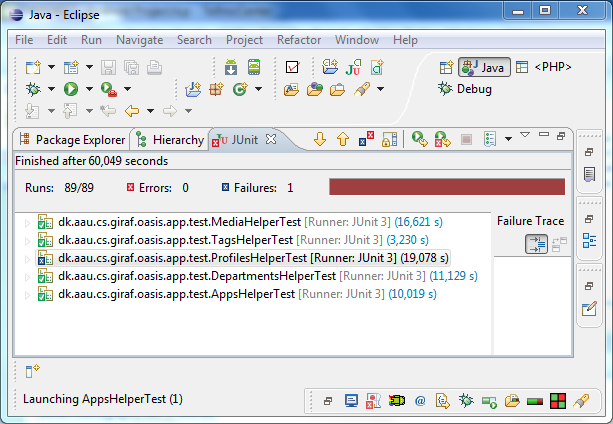
\includegraphics[width=\textwidth]{Images/unit_testing/all_tests.PNG}
	\caption{The result from all the performed unit tests.}
	\label{fig:all_tests}
\end{figure}

The test that failed is \texttt{testGetChildrenByDepartmentAndSubDepartments()} and the result can be seen in Figure \vref{fig:profile_helper_tests}.

\begin{figure}[H]
	\centering
		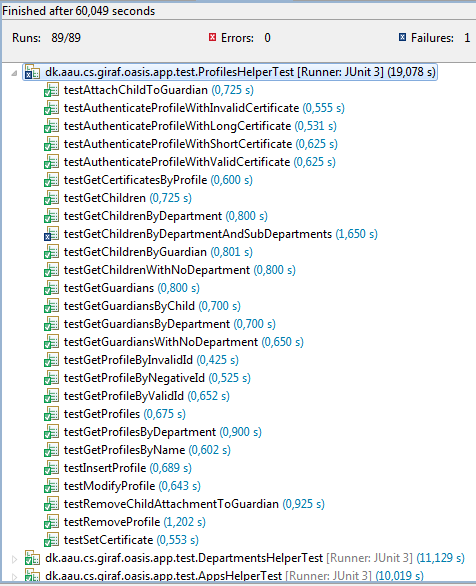
\includegraphics[width=\textwidth]{Images/unit_testing/profile_helper_tests.PNG}
	\caption{The result from the \texttt{profilesHelper} tests.}
	\label{fig:profile_helper_tests}
\end{figure}

The individual results for the rest of the test suite can be seen in Appendix \vref{app:unitTestResults}.